\chapter{\IfLanguageName{dutch}{Stand van zaken}{State of the art}}%
\label{ch:stand-van-zaken}

% Tip: Begin elk hoofdstuk met een paragraaf inleiding die beschrijft hoe
% dit hoofdstuk past binnen het geheel van de bachelorproef. Geef in het
% bijzonder aan wat de link is met het vorige en volgende hoofdstuk.

% Pas na deze inleidende paragraaf komt de eerste sectiehoofding.
\section{Inleiding}

%Dit hoofdstuk bevat je literatuurstudie. De inhoud gaat verder op de inleiding, maar zal het onderwerp van de bachelorproef *diepgaand* uitspitten. De bedoeling is dat de lezer na lezing van dit hoofdstuk helemaal op de hoogte is van de huidige stand van zaken in het onderzoeksdomein. Iemand die niet vertrouwd is met het onderwerp, weet nu voldoende om de rest van het verhaal te kunnen volgen, zonder dat die er nog andere informatie moet over opzoeken \autocite{Pollefliet2011}.
%
%Je verwijst bij elke bewering die je doet, vakterm die je introduceert, enz.\ naar je bronnen. In \LaTeX{} kan dat met het commando \texttt{$\backslash${textcite\{\}}} of \texttt{$\backslash${autocite\{\}}}. Als argument van het commando geef je de ``sleutel'' van een ``record'' in een bibliografische databank in het Bib\LaTeX{}-formaat (een tekstbestand). Als je expliciet naar de auteur verwijst in de zin (narratieve referentie), gebruik je \texttt{$\backslash${}textcite\{\}}. Soms is de auteursnaam niet expliciet een onderdeel van de zin, dan gebruik je \texttt{$\backslash${}autocite\{\}} (referentie tussen haakjes). Dit gebruik je bv.~bij een citaat, of om in het bijschrift van een overgenomen afbeelding, broncode, tabel, enz. te verwijzen naar de bron. In de volgende paragraaf een voorbeeld van elk.
%
%\textcite{Knuth1998} schreef een van de standaardwerken over sorteer- en zoekalgoritmen. Experten zijn het erover eens dat cloud computing een interessante opportuniteit vormen, zowel voor gebruikers als voor dienstverleners op vlak van informatietechnologie~\autocite{Creeger2009}.
%
%Let er ook op: het \texttt{cite}-commando voor de punt, dus binnen de zin. Je verwijst meteen naar een bron in de eerste zin die erop gebaseerd is, dus niet pas op het einde van een paragraaf.
%
%\begin{figure}
%  \centering
%  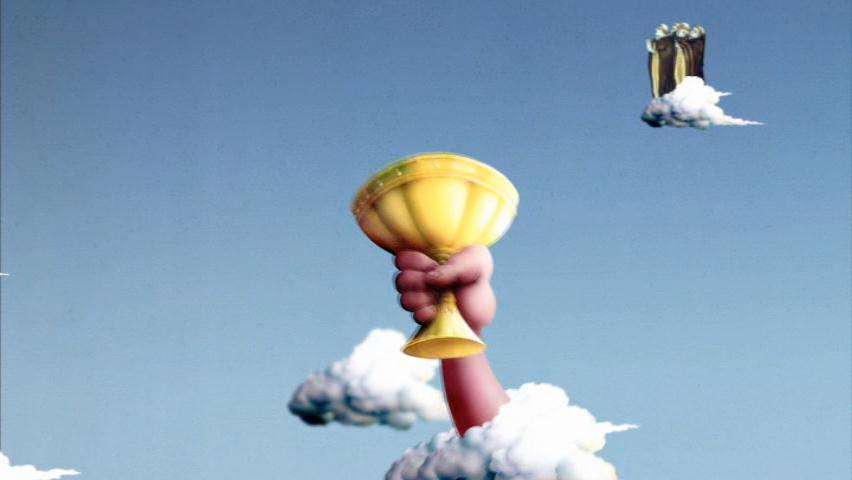
\includegraphics[width=0.8\textwidth]{grail.jpg}
%  \caption[Voorbeeld figuur.]{\label{fig:grail}Voorbeeld van invoegen van een figuur. Zorg altijd voor een uitgebreid bijschrift dat de figuur volledig beschrijft zonder in de tekst te moeten gaan zoeken. Vergeet ook je bronvermelding niet!}
%\end{figure}

%\begin{listing}
%  \begin{minted}{txt}
%    import pandas as pd
%    import seaborn as sns
%
%    penguins = sns.load_dataset('penguins')
%    sns.relplot(data=penguins, x="flipper_length_mm", y="bill_length_mm", hue="species")
%  \end{minted}
%  \caption[Voorbeeld codefragment]{Voorbeeld van het invoegen van een codefragment.}
%\end{listing}

%\lipsum[7-20]

%\begin{table}
%  \centering
%  \begin{tabular}{lcr}
%    \toprule
%    \textbf{Kolom 1} & \textbf{Kolom 2} & \textbf{Kolom 3} \\
%    $\alpha$         & $\beta$          & $\gamma$         \\
%    \midrule
%    A                & 10.230           & a                \\
%    B                & 45.678           & b                \\
%    C                & 99.987           & c                \\
%    \bottomrule
%  \end{tabular}
%  \caption[Voorbeeld tabel]{\label{tab:example}Voorbeeld van een tabel.}
%\end{table}
\section{Facilitair beheer}
Facilitair beheer (FM) is een interdisciplinair vakgebied dat de coördinatie van mensen, processen en ruimtes omvat om welzijn en efficiëntie binnen organisaties te verbeteren (ISO 41011:2018) \autocite{jaouhari2023we}. 

\section{facilitaire diensten van HOGENT}
Het centrale punt voor het beheer van facilitaire diensten op HOGENT heeft als locatie de campus Mercator. Hier wordt de informatie verzameld en gemonitord van alle campusen binnen het gebouwbeheersysteem. Voor deze bachelorproef wordt er dieper ingegaan op de campus Schoonmeersen.

\subsection{Campus Schoonmeersen}
Op de campus Schoonmeersen zijn er 2 platformen om de informatie te verzamelen van de facilitaire diensten. Deze platformen zijn Johnson controls Metasys en Schneider's Schneider Electric. Metasys is in gebruik in gebouw D (GSCHD) zie figuur 2.1 en Scneider Electric is in gebruik in de gebouwen B (GSCHB), C (GSCHC), P (GSCHP) en de HOGENT Sporthal zie figuur 2.2 \autocite{Venneman2019}.

\begin{figure}
    \centering
    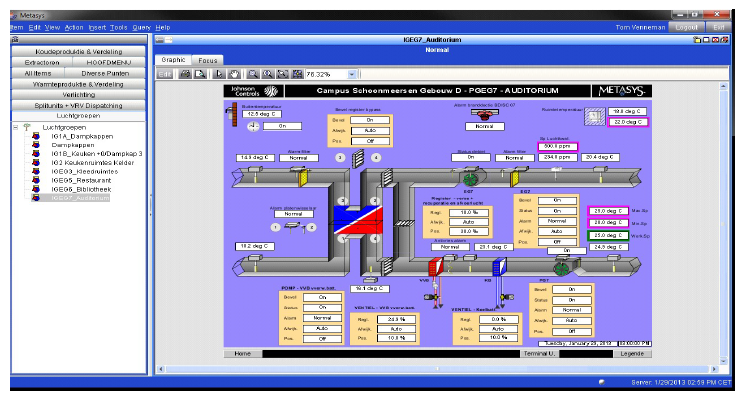
\includegraphics[width=0.8\textwidth]{metasys.png}
    \caption[metasys bron. HOGENT gebouwbeheersysteem (Metasys)]{\label{fig:metasys}metasys bron. HOGENT gebouwbeheersysteem (Metasys), luchtgroep gebouw D}
\end{figure}
\begin{figure}
    \centering
    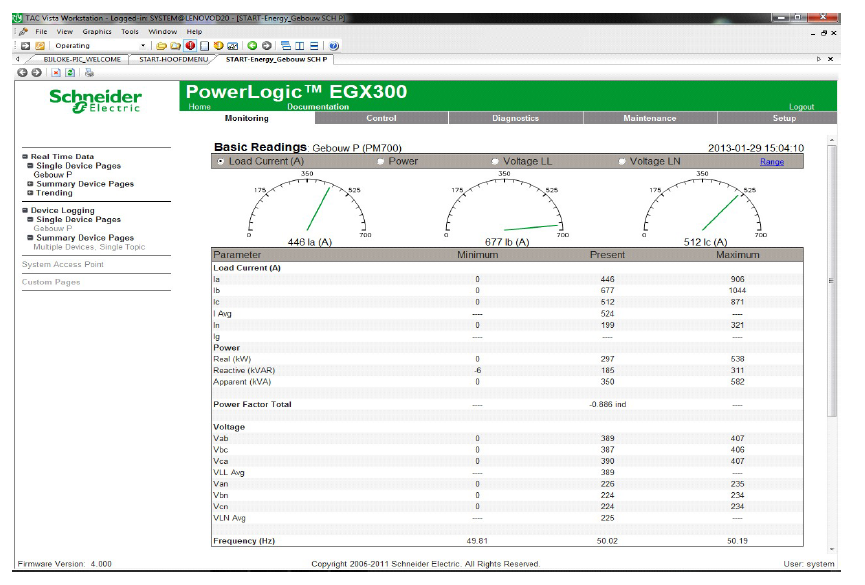
\includegraphics[width=0.8\textwidth]{Schneider_Electric.png}
    \caption[Schneider Electric. bron. HOGENT gebouwbeheersysteem (Schneider Electric)]{\label{fig:schneiderelectric}Schneider Electric. bron. HOGENT gebouwbeheersysteem (Schneider Electric), weergave van het stroom- en spanningsverbruik en het vermogen van het gebouw P op de campus Schoonmeersen.}
\end{figure}

\subsection{Xenta modules}
In de gebouwen wordt er gebruik gemaakt van Xenta modules. Xenta module 401 is telkens de hoofdregelaar voor de systemen. Hieraan zijn dan telkens maximaal 10 input output apparaten verbonden en deze staan dan in voor het verzamelen van de gegevens van de diverse metingen. Er zijn verschillende soorten van input output apparaten zoals te zien in figuur 2.3. Digitale input en output apparaten hebben 2 vaste staten zoals uit en aan. Een thermistor is een weerstandsthermometer, of een resistor waarvan de weerstand afhankelijk is van de temperatuur. Analoge apparaten gebruiken continue signalen die variëren in grootte, zoals spanning, stroom of weerstand. Universele apparaten zijn apparaten die zowel kunnen dienen als digitale input en output en als analoge output.

\begin{figure}
  \centering
  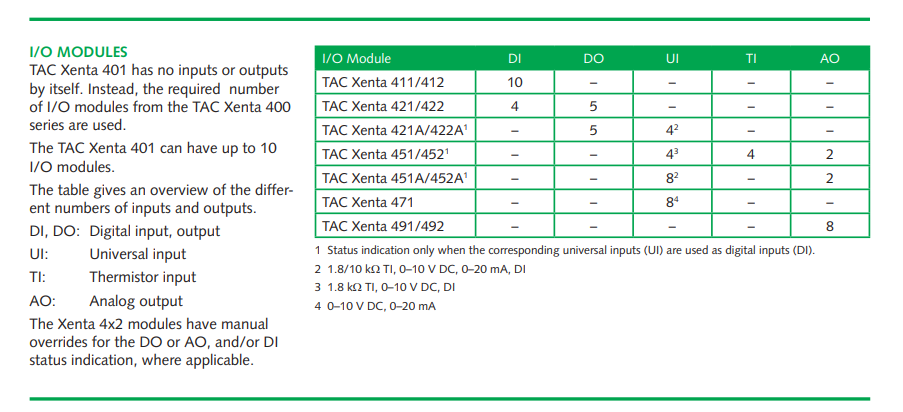
\includegraphics[width=0.8\textwidth]{tabel_XentaModules.png}
  \caption[Xenta modules. bron. Schneider Electric documenten]{\label{fig:xentamodules}Xenta modules. bron. Schneider Electric documenten}
\end{figure}


%\subsection{Spacelogic}
%De gebouwen op de campus Schoonmeersen maken gebruik van een Spacelogic controller AS-P om te communiceren via een toegewezen ip adres.

% TO DO: foto's bijzetten
\subsection{Verlichting}
Op het hoofdscherm van het systeem bevindt zich een schakelaar waarmee de verlichting van de gebouwen vanuit Mercator kan worden aangestuurd. De verlichting werkt volgens een vooraf ingesteld tijdschema. Binnen de gebouwen mogen de lichten aanstaan op de volgende tijden:

\begin{itemize}
    \item \textbf{Maandag tot en met vrijdag:} 05:30 -- 22:00
    \item \textbf{Zaterdag:} 07:00 -- 19:00
\end{itemize}

Voor de buitenverlichting geldt een iets ruimer tijdschema:

\begin{itemize}
    \item \textbf{Maandag tot en met vrijdag:} 05:30 -- 22:15
    \item \textbf{Zaterdag:} 07:20 -- 19:20
\end{itemize}

Naast tijdsinstellingen wordt ook de helderheid gemeten om te bepalen of verlichting noodzakelijk is. Voor binnenverlichting geldt een drempelwaarde van $60.000$ lux, terwijl deze voor buitenverlichting op $60$ lux ligt. Wanneer de helderheid onder deze grenswaarden komt, kan de verlichting worden ingeschakeld.

Voor gebouwen waarbij de verlichting niet vanuit Mercator kan worden aangestuurd, gebeurt de bediening handmatig.

\subsection{HVAC (Heating, Ventilation, and Air Conditioning)}
Gebouw T beschikt over het meest geavanceerde HVAC-systeem op de campus Schoonmeersen en dient als referentie voor de overige gebouwen. De warmteproductie binnen de gebouwen wordt voornamelijk verzorgd door ketels. In Gebouw T is daarnaast een warmtepomp geïnstalleerd, wat zorgt voor een efficiëntere en flexibelere regeling.

De werking van de ketels is gebaseerd op het aantal draaiuren, wat vooral van belang is voor onderhoudsplanning. Wanneer een warmtepomp aanwezig is, fungeert deze als \textbf{primaire} warmtebron, terwijl de ketels als \textbf{secundaire} warmtevoorziening dienen.

De warmtepomp hanteert specifieke temperatuursinstellingen:

\begin{itemize}
    \item \textbf{Verwarming (heating):} Ingeschakeld bij een temperatuur onder $16°C$
    \item \textbf{Neutrale stand:} Tussen $16°C$ en $18°C$
    \item \textbf{Koeling (cooling):} Geactiveerd bij temperaturen boven $18°C$
    \item \textbf{Vorstbescherming:} In de winter schakelt het systeem automatisch over op verwarming wanneer de temperatuur onder $5°C$ daalt
\end{itemize}

\subsubsection{Zone-indeling en temperatuurregeling}
De gebouwen zijn opgedeeld in verschillende verwarmingskringen, waarbij een kring een verzameling radiatoren omvat. In oudere gebouwen vormen deze kringen het eindpunt van de regeling, terwijl Gebouw T daarnaast nog extra \textbf{zoneregelaars} per lokaal heeft. Hierdoor is een meer gedetailleerde temperatuurregeling mogelijk.

De verwarmingskringen werken volgens een \textbf{tijdsschema}:

\begin{itemize}
    \item \textbf{Maandag tot en met zaterdag:} 05:30 -- 17:30
    \item \textbf{Donderdag:} Uitgebreide werking tot 19:30
    \item \textbf{Nachttemperatuur:} 16 °C
    \item \textbf{Overdag:} De binnenruimtetemperatuur wordt automatisch aangepast op basis van de buitentemperatuur, met een gemiddelde richtwaarde van 19 °C
\end{itemize}

Dankzij de zoneregelaars kan de temperatuur per lokaal worden aangepast. Hierbij wordt rekening gehouden met aanwezigheidssensoren die de ruimtestatus bepalen:

\begin{itemize}
    \item \textbf{Unoccupied:} Ruimte is niet in gebruik $\rightarrow$ 16 °C
    \item \textbf{Standby:} Ruimte is actief, maar leeg $\rightarrow$ 18 °C
    \item \textbf{Occupied:} Ruimte is in gebruik $\rightarrow$ 19 °C
\end{itemize}

\subsubsection{Ventilatie}
De ventilatie wordt geregeld per luchtgroep. Buitenlucht wordt via een warmtewiel en een warmtebatterij (kleine warmtekring) gefilterd en opgewarmd voordat het via ventilatoren naar binnen wordt gebracht. De ventilatie werkt op basis van zowel een tijdsklok als een \textbf{drukregeling}, waarbij de druk binnen de waarden van $400$ Pa tot $500$ Pa blijft.

In Gebouw T kunnen de zoneregelaars ook de ventilatie aansturen. Dit gebeurt op basis van \textbf{CO$_2$-concentratie}. Wanneer de CO$_2$-waarde de drempel van $800$ ppm overschrijdt, worden de regelkleppen automatisch meer geopend om extra ventilatie toe te laten.

Elk van deze regelmodules verzamelt en logt verschillende meetwaarden, waardoor temperatuur- en ventilatiegegevens grafisch kunnen worden weergegeven.

\subsubsection{Verwarmingsperiode}
Het stookseizoen loopt doorgaans van \textbf{oktober tot april/mei}, afhankelijk van de buitentemperaturen en de verwarmingsbehoefte.

\subsection{Storingen en Monitoring}
Storingen worden in \textbf{realtime} geregistreerd en weergegeven in Mercator via een overzichtelijke lijst. Hierdoor kunnen bekende problemen direct worden gemonitord en kunnen storingen snel worden opgelost voordat ze een impact hebben op het comfort binnen de gebouwen.

\section{Vergelijking 4G en 5G}
Het verschil tussen 4G en 5G in facilitair beheer ligt in de infrastructuur en middelenbeheer. 5G biedt flexibelere en efficiëntere infrastructuur dankzij virtualisatie wat zorgt voor schaalbaarheid en minder handmatige interventie \autocite{degambur2021resource}. 5G introduceert een verbeterde netwerkcapaciteit, betrouwbaarheid en efficiëntie, met lagere latentie en lager energieverbruik ten opzichte van 4G. De nadruk ligt op hoge snelheden en het verbinden van meerdere apparaten tegelijkertijd \autocite{mihret20214g}. De integratie van 5G technologie in het facilitair beheer van slimme gebouwen biedt voordelen voor efficiëntie, connectiviteit en veiligheid. Hoewel uitdagingen zoals hoge investeringskosten en complexe integratie bestaan, maar de voordelen van verbeterde duurzaamheid, efficiëntie en comfort overtreffen deze uitdagingen \autocite{Markogiannaki2023}. Private 5G netwerken bieden bedrijven en organisaties een veilig, flexibel en schaalbaar alternatief voor publieke 5G netwerken. Private 5G netwerken maken het mogelijk om data veilig en autonoom te delen zonder de openbare internetinfrastructuur te gebruiken \autocite{eswaran2023private}.

5G biedt hogere datasnelheden, lagere latentie en ondersteuning voor veel meer verbonden apparaten  dan 4G dankzij mmWave-technologie, massive MIMO en ultra-dense netwerken \autocite{Hui_2020}.


\section{Smart campussen}
\textcites{Min_Allah_2020,AbuAlnaaj2016,Ahmed2022} beschrijven hoe smart campussen geavanceerde technologieën zoals het Internet of Things (IoT), 5G-connectiviteit en kunstmatige intelligentie (AI) gebruiken om onderwijsinstellingen efficiënter, duurzamer en gebruiksvriendelijker te maken. Deze technologieën verbeteren niet alleen de leeromgeving, maar optimaliseren ook energiebeheer, beveiliging en operationele efficiëntie \autocite{Correia2022}. Een belangrijke uitdaging bij de implementatie van smart campus-technologieën is de hoge kosten, cyberveiligheidsrisico’s en de noodzaak van een geïntegreerde infrastructuur \autocite{Liu_2022}. Desondanks tonen studies aan dat de voordelen, zoals energiebesparing en verhoogde veiligheid, opwegen tegen deze uitdagingen \autocite{AbuAlnaaj2016}.

\section{IoT en 5G in smart campussen, steden en gebouwen}

\textcite{Bilardo_2021} stelt dat IoT en 5G een cruciale rol spelen in de ontwikkeling van slimme steden en campussen door real-time monitoring en communicatie tussen apparaten mogelijk te maken. Hierdoor kunnen systemen zoals verlichting, klimaatregeling en beveiliging automatisch worden aangepast aan de behoeften van gebruikers, wat leidt tot een efficiënter energiegebruik en lagere operationele kosten \autocite{Polin2023}. De integratie van IoT binnen smart cities bevordert niet alleen duurzaamheidsdoelstellingen, maar verbetert ook de kwaliteit van leven door slimmere mobiliteit en infrastructuur \autocite{Chew2020}. Toch brengt de implementatie van IoT beveiligingsrisico’s met zich mee, zoals gegevenslekken en cyberaanvallen, wat een belangrijk aandachtspunt blijft voor beleidsmakers en technologieleveranciers \autocite{Trivedi2017}.

\section{HVAC-systemen en slim energiebeheer}

\textcite{Correia2022} legt uit dat efficiënte HVAC-systemen (verwarming, ventilatie en airconditioning) essentieel zijn voor slimme gebouwen en campussen, aangezien ze verantwoordelijk zijn voor een groot deel van het energieverbruik. Door AI en IoT te combineren, kunnen deze systemen worden geoptimaliseerd om energie te besparen zonder dat dit ten koste gaat van het comfort van gebruikers \autocite{Min_Allah_2020}. Geavanceerde algoritmes en machine learning spelen een grote rol bij het voorspellen van energieverbruik en het automatisch aanpassen van HVAC-instellingen om piekbelasting te verminderen \autocite{Khoa2020}. Daarnaast helpt IoT-technologie bij het continu monitoren en onderhouden van HVAC-systemen, waardoor storingen en inefficiëntie sneller kunnen worden opgespoord en verholpen \autocite{Zhang2022}.

\section{Slimme verlichting}

\textcite{Poyyamozhi2024} stelt dat slimme verlichting in zowel binnen- als buitenomgevingen bijdraagt aan energie-efficiëntie en verhoogd gebruikerscomfort. In gebouwen maken slimme verlichtingssystemen gebruik van sensoren en AI om de lichtsterkte en kleurtemperatuur aan te passen op basis van de aanwezigheid van personen en de hoeveelheid natuurlijk licht \autocite{Wang2024}. In buitenomgevingen, zoals smart cities, helpt geautomatiseerde straatverlichting energie te besparen door middel van bewegingsdetectie en connectiviteit met andere stadsnetwerken \autocite{Huseien_2022}. Hierdoor wordt niet alleen het energieverbruik verminderd, maar ook de veiligheid en bruikbaarheid van stedelijke ruimtes verbeterd.

Door de integratie van IoT, 5G en AI kunnen smart campussen en gebouwen op een duurzamere en efficiëntere manier functioneren. Hoewel er uitdagingen zijn zoals kosten en beveiligingsrisico’s, wegen de voordelen op lange termijn ruimschoots op tegen deze obstakels.






